\documentclass[10pt, colorlinks=true, urlcolor=blue]{beamer}

% Themes and colors for a professional look
\usetheme{Madrid}
\usecolortheme{seagull}
\setbeamercolor{title}{fg=white,bg=blue!80!black}
\setbeamercolor{frametitle}{fg=white,bg=blue!70!black}
\setbeamercolor{block title}{fg=white,bg=blue!80!black}
\setbeamercolor{block body}{bg=blue!5!white}


% Set hyperlink colors
\hypersetup{
    colorlinks=true,    % Enable colored links
    urlcolor=blue,      % Color for URLs
    linkcolor=blue      % Color for internal links (optional)
}

\usepackage{minted}

\title{Mutability in the Python Data Model}
\author{Bas Terwijn}
\titlegraphic{
\includegraphics[width=0.6\textwidth]{figures/uva.png}}
\date{\today}

\begin{document}

\begin{frame}
    \titlepage
\end{frame}

\begin{frame}{Content}

  The \href{https://docs.python.org/3/reference/datamodel.html}{\texttt{Python Data Model}} it a large topic, we will focus only on:
  \begin{itemize}
  \item Mutability of Types
  \item Coping Mutable Values
  \end{itemize}

  \vspace{2em}
  
  These concepts are fundamental to Python programming.
  \begin{itemize}
    \item without a solid understanding you cannot avoid certain bugs
  \end{itemize}

  \vspace{2em}
  
  To help build a solid understanding we will demonstrate visualization tools:
  \begin{itemize}
  \item \href{https://pypi.org/project/memory-graph/}{\texttt{Memory\_Graph}}
  \item \href{https://pythontutor.com/}{\texttt{Python Tutor}}
  \end{itemize}

  \vspace{2em}

  We will finish with an exercise with which you can test your understanding.
\end{frame}


\begin{frame}{Immutable and Mutable Types}
    \begin{block}{Python Types}
        Python has two distinct categories of types: Immutable, Mutable
    \end{block}

    \vspace{3em}
    
    \textbf{Immutable Types:} \texttt{bool}, \texttt{int}, \texttt{float}, \texttt{complex}, \texttt{str}, \texttt{tuple}, \texttt{bytes}, \texttt{frozenset} \\
    
    \vspace{-0.8em}
    A value of an immutable type \textbf{cannot} be changed in place. \\
    Therefore, \textbf{a} copy is made when you change it. \\
    
    \vspace{2.5em}
    
    \textbf{Mutable Types:} \texttt{list}, \texttt{set}, \texttt{dict}, \texttt{classes}, \dots (most other types) \\
    
    \vspace{-0.8em}
    A value of a mutable type \textbf{can} be changed in place. \\
    \textbf{No} copy is made when you change it.
    
\end{frame}

\begin{frame}[fragile]
  \frametitle {Sharing Mutable Values}
  When two variable share a \textbf{mutable} value, changing one changes the other.
  \vspace{1em}
\begin{columns}
  \column{0.3\textwidth}
  \begin{minted}[fontsize=\small]{python}
           a = [4, 3, 2]
           b = a
           a += [1]
    \end{minted}
  \column{0.7\textwidth}
    \begin{center}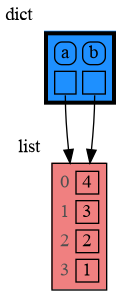
\includegraphics[width=0.25\textwidth]{figures/sharing.png}\end{center}
\end{columns}
\vspace{1em}
Sometimes you want this, but when you don't you have to make a copy so that each variable has its own independent value.
\end{frame}


\begin{frame}[fragile]
  \frametitle {Copying Mutable Values}
  When ``copying'' a \textbf{mutable} value, consider the amount of sharing you need:
  \vspace{-1em}
\begin{columns}
  \column{0.4\textwidth}
  \begin{minted}[fontsize=\small]{python}
      a = [[1, 2], ['x', 'y']]
      c1 = a
      c2 = copy.copy(a)
      c3 = copy.deepcopy(a)
    \end{minted}
  \column{0.6\textwidth}
    \begin{center}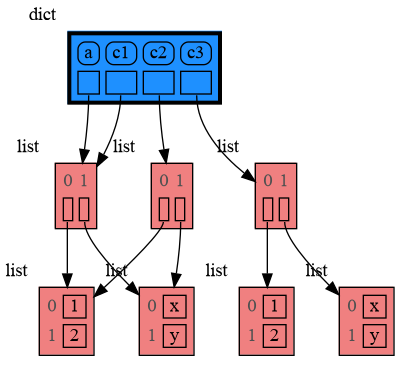
\includegraphics[width=0.7\textwidth]{figures/copy.png}\end{center}
\end{columns}
    \begin{itemize}
        \item \textbf{c1: Assignment,} nothing is copied, all the values are shared
        \item \textbf{c2: Shallow Copy,} only the value referenced by the first reference is copied, all the underlying values are shared
        \item \textbf{c3: Deep Copy,} all the values are copied, nothing is shared
        \item \ \ \, \,\, \textbf{Custom Copy,} alternatively write your own copy logic
    \end{itemize}
\end{frame}

\begin{frame}{Function Call}
  Calling a function with a \textbf{mutable} value might change that value.
  \begin{itemize}
  \item If you don't want that, make a copy.
  \end{itemize}
  \begin{center}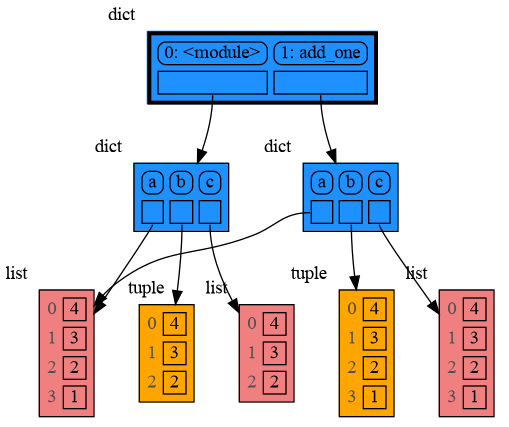
\includegraphics[width=0.65\textwidth]{figures/function_call.png}\end{center}
\end{frame}

\begin{frame}{Memory\_Graph Debugger Setup}
  install
  debugger, vscode
  blocking pdf reader, different format
\end{frame}

\begin{frame}{Memory\_Graph Non-Debugger Setup}
  insert code where to show/render
\end{frame}

\begin{frame}{Python Tutor}
  example add\_one
  Pros:
  \begin{itemize}
  \item no installation or setup required
  \item can debug backwards
  \item widely used
  \item support multiple programming languages
  \end{itemize}
  Cons:
  \begin{itemize}
  \item runs in a webbrower
  \item limited program: size, runtime, memory usage
  \item can only import standard library modules
  \item no reading/writing files and command-line arguments 
  \end{itemize}
\end{frame}

\begin{frame}{Example: Recursion}
  factorial
  power\_set
\end{frame}

\begin{frame}{Exercise}
  mental model
\end{frame}


\end{document}
